\section{Teori}
Det här är\footfullcite{einstein} teori \cite{einstein}.
\subsection{Underrubrik}
Hänvisning till \cref{eq:namn}
\begin{equation} \label{eq:namn}
    E=m \cdot c^2.
\end{equation}

Hänvisning till \cref{tab:namn}.
\begin{table}[H]
\centering
\caption{Tabellhuvud.}
\begin{tabular}{ l l l } \toprule
\textbf{Symbol} & \textbf{Storhet} & \textbf{Dimension} \\
\midrule
    $E$ & Energi & \si{M.L^2.T^{2}} \\
    $m$ & Massa &\si{M} \\
    $c$ & Ljusets hastighet & \si{L.T^{-1}} \\
\bottomrule 
\end{tabular} \label{tab:namn}
\end{table}

Hänvisning till \cref{fig:namn}.
\begin{figure} [H]
    \centering 
    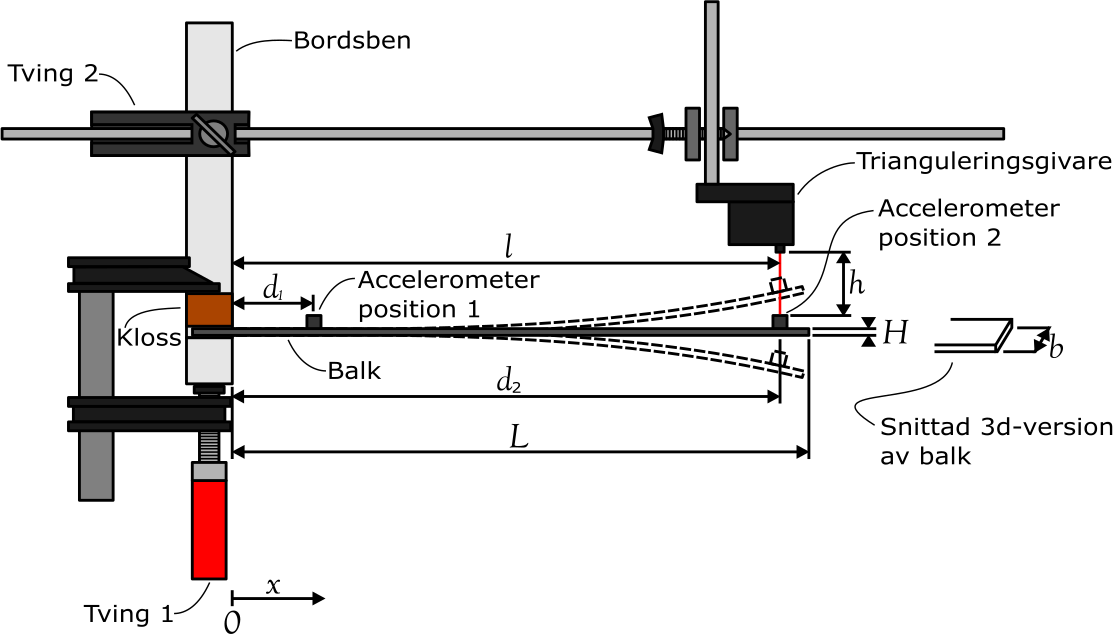
\includegraphics[width=0.5\textheight]{experiment_uppstallning.png}
    \caption{Beskrivande text.}
    \label{fig:namn}
\end{figure}